This Bachelor's Thesis aligns directly with the University of the Basque Country's (UPV/EHU) EHUagenda 2030 for sustainable development. Specifically, this research contributes fundamentally to Sustainable Development Goal (SDG) 9: Industry, Innovation, and Infrastructure, which is one of the core SDGs formally adopted by UPV/EHU.  

Within the framework of SDG 9, UPV/EHU emphasizes United Nations Target 9.5, which aims to enhance scientific research, upgrade the technological capabilities of industrial sectors, and encourage innovation. As modern manufacturing and technological industries increasingly rely on Artificial Intelligence to automate processes and ensure quality control—such as the defect detection applications represented by the NEU-DET dataset—the underlying computational infrastructure must be both highly scalable and impeccably secure.  

Decentralized Federated Learning (DFL) represents a critical technological leap in this domain. It allows multiple industrial entities to collaboratively train robust machine learning models without ever centralizing or exposing their sensitive, proprietary data. However, this infrastructure upgrade introduces severe structural vulnerabilities. By removing the central server, DFL networks become susceptible to localized backdoor poisoning attacks, where malicious actors attempt to embed hidden, destructive behaviors into the global model.

This thesis directly addresses this vulnerability by mathematically evaluating how specific network topologies, particularly community-based structures like the Stochastic Block Model, can act as natural "firewalls." By proving that these architectures can structurally suppress continuous adversarial attacks without sacrificing model utility, this research provides the essential scientific foundation needed to build the resilient, secure, and sustainable AI infrastructures required by modern industry, fully supporting the innovation mandates of SDG 9.

\begin{figure}[ht]
  \centering
  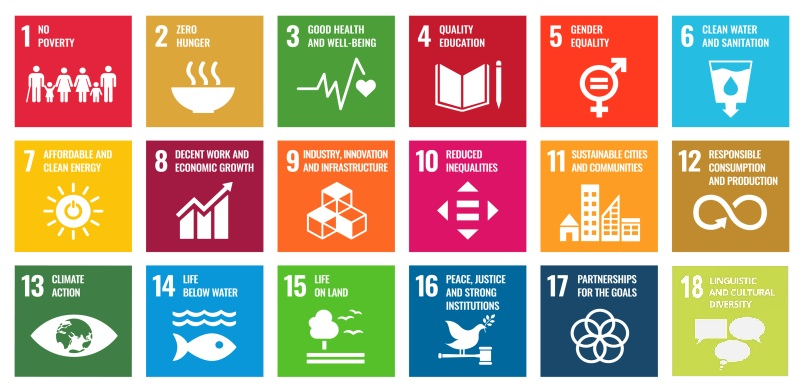
\includegraphics[width=\linewidth]{figures/SDG.jpg}
  \caption{SDG 2030}
  \label{fig:SDG_2030}
\end{figure}